% arara: pdflatex
% arara: nomencl
% arara: bibtex
% arara: pdflatex
\documentclass[12pt]{report}
\usepackage{graphicx}
\usepackage[margin=0.5in]{geometry}
\usepackage{	array,
			booktabs,
			cite,
			enumitem,
			epstopdf,
			fancyhdr,
			graphicx,
			lipsum,
			lscape,
			mathtools,
			mcode,
			nomencl,			
			parallel,
			rotating,
			soul,
			titlesec,
			wrapfig,
			}
\usepackage{soul}
\usepackage[toc,page]{appendix}
\usepackage{mcode}
\graphicspath{ {./images/} } % Graphics Path
\renewcommand{\abstractname}{Project Goal}
\usepackage[parfill]{parskip}
\makenomenclature
\renewcommand{\chaptername}{Section}

\bibliographystyle{plain}

\setcounter{tocdepth}{6}
\setcounter{secnumdepth}{6}
\setcounter{chapter}{0}
\setlength{\abovetopsep}{4pt}
\setlength{\heavyrulewidth}{1.5pt}

% Margin Setup

\addtolength{\oddsidemargin}{.3in}
\addtolength{\evensidemargin}{.5in}
\addtolength{\topmargin}{.2in}
\addtolength{\textwidth}{-.6in}
\addtolength{\textheight}{-.4in}

\title{The Design, Development and Implementation of a Scanning Fabry-Perot Interferometer}
\author{David M Houston\\
		Oregon Institute of Technology\\\\
		}

		
\nomenclature{$F^*$}{The finesse of the resonant cavity}%
\nomenclature{$c$}{The speed of light}%
\nomenclature{$\lambda$}{The wavelength of light in nanometers}%
\nomenclature{$R$}{The reflectivity of the mirrors}%
\nomenclature{$L$}{The length of the resonant cavity}%
\nomenclature{$F^*$}{The finesse of the resonant cavity}%
\nomenclature{$\Delta~v$}{The free spectral range}%

\begin{document}
\maketitle
\tableofcontents
\listoffigures
\listoftables

% Project Goals

\begin{abstract}
The goal of the project is to design, build, and implement a scanning mirror Fabry-Perot Interferometer. This device characterizes the spectral content of a laser beam. It will have a finesse of  and frequency spectral range of 3.748 GHz with a resolution of 24 MHz. 
A piezoelectric device will change the spacing of the mirrors, allowing scanning across the entire free spectral range. A driver will provide a controllable voltage signal to the piezoelectric device. The spectral frequency content will be captured by a photodetector and amplified by an adjustable transimpedance amplifier with a gain range of 50dB. A computer will process, display, and store this data locally on its hard disk.
\end{abstract}

% Background Section
%\section{Background}
\chapter[Background]{The Fabry-Perot Interferometer}
The scanning Fabry-Perot Interferometer (sFPI) allows high-resolution optical spectroscopy. An example of this device is the Spectra Physics 470-04 Interferometer (SP-470-04), which is "a mode degenerate, spherical mirror, Fabry-Perot interferometer". It has a confocal resonant cavity with a minimum finesse of 150 and a free spectral range (FSR) of 8 GHz. This is calculated by Eq.~\ref{finesse}~\cite{spectraphysics470}. 

% finesse
\begin{equation}
F^* = \pi\frac{\sqrt{R}}{1-R}
\label{finesse}
\end{equation}

The sFPI ``can be used as a scanning spectrum analyzer..., as a static fringe interferometer, or as a tunable optical filter...''~\cite{spectraphysics470}. The SP-470-04 is comprised of a resonant cavity, capable of scanning, a driver, and a photo-detection setup for data analysis. The resonant cavity is constructed of a confocal mirror setup with an auxiliary lens as seen in Figures~\ref{fig:mirrorsetup} and~\ref{fig:beamdia}~\cite{hercher}.\\

% Mirror Setup
\begin{figure}[h!]
  \centering
	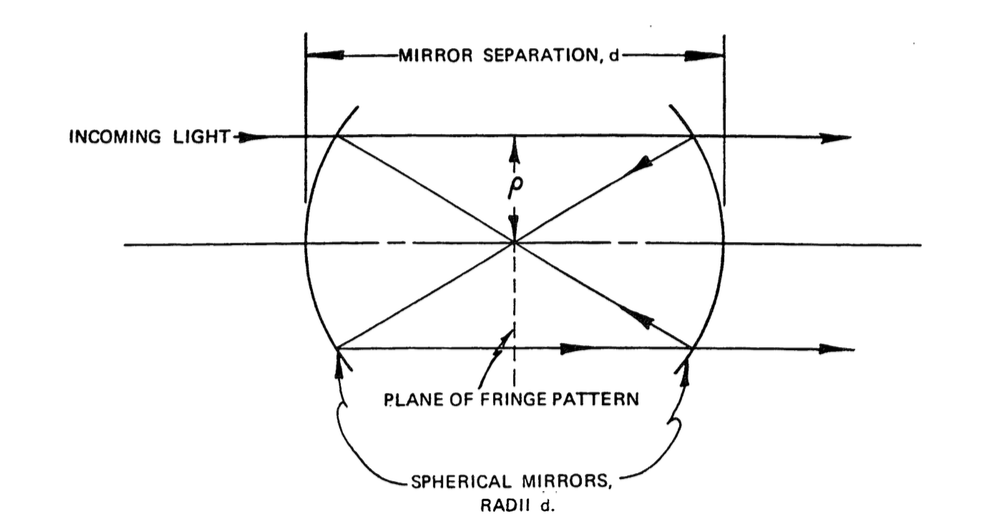
\includegraphics[width=6in]{Fig1A.png}\\
	\caption[Resonant Cavity Setup]{Resonant Cavity Mirror Setup~\cite{spectraphysics470}}
	\label{fig:mirrorsetup}
\end{figure}

% Beam Diameters
\begin{figure}[h!]
  \centering
	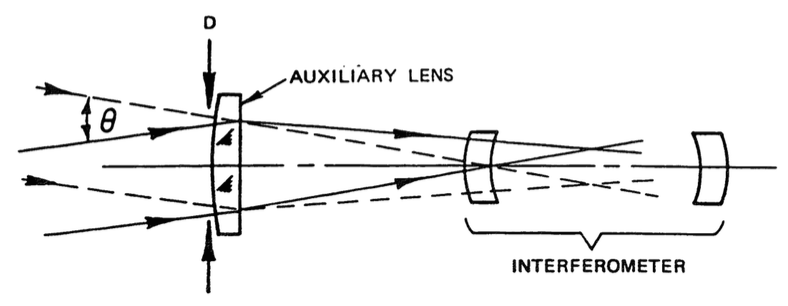
\includegraphics[width=6in]{Fig2A.png}\\
	\caption[Auxiliary Lens Setup]{Incident Beam Diameter and Angular Divergence with Auxiliary Lens~\cite{spectraphysics470}}
	\label{fig:beamdia}
\end{figure}


The first Fabry-Perot Interferometer was built using plane mirrors so as to be manipulated by changing their ``relative orientation and particularly to render them rigorously parallel". To properly calibrate the device, the mirrors were set to a calibrated distance which corresponded with the ``first resolution of the two yellow lines of mercury"~\cite{fabry-perot}. This design has changed over the years with the developments of the spherical mirror Fabry-Perot Interferometer (sFPI) and the internally coupled Fabry-Perot Interferometer (icFPI), which is simply a modification of the sFPI~\cite{hercher}~\cite{reich}. The sFPI is free from considerations due to mode matching and has increased optical power making it more efficient for higher resolution spectroscopy. Because the sFPI is more sensitive to changes in the mirror separations, changing the geometry of the resonant cavity allows for the scanning through the FSR.~\cite{hercher}. \newline


\noindent There are two systems that can be used for changing the length of the resonant cavity. A pressure scanning system is used for scanning by a pressure differential to expand and contract the resonant cavity; however, its primary use is for static ultra-high resolution spectroscopy. The piezo-electrical scanning system, used by applying electrical charge, is utilized in spectrum analysis, tunable narrow bandpass filtering, and fringe interferometry~\cite{hercher}. The piezo-electric device operates as an transducer that "when an electric field is applied... deformation $(\Delta L)$ or strain $(\Delta L/L)$ arises". It has a corresponding impedance layout, that can be modeled using a resistor, capacitor, inductor circuit structure, with components corresponding to the piezoelectric motion and electrostatic capacitance \cite{piezo}. To produce the scanning effect a saw-tooth electric signal is applied across the piezoelectric device causing a change in length of the cavity~\cite{piezo}~\cite{hercher}.\newline


The current driver, a Spectra Physics Model 476 Scanning Interferometer, produces a variable saw-tooth signal, as seen in Figure~\ref{fig:outputramp}. It has the capabilities of producing a max voltage of $300 V$ or $1 kV$ with a variable amplitude, offset, and frequency for each condition~\cite{sfpidriver}.  

\begin{figure}[h!]
	\centering
	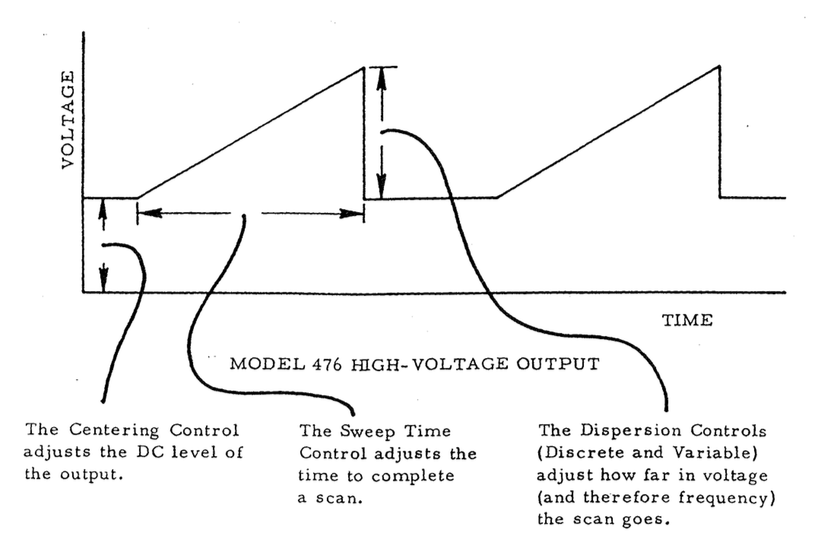
\includegraphics[width=6in]{driver.png}
	\caption[Spectra Physics Model 476 High-Voltage Output]{Spectra Physics Model 476 High-Voltage Output~\cite{sfpidriver}}
	\label{fig:outputramp}
\end{figure}

The SP-476 uses Op-Amps, switches, varistors, and BJT's (Figure~\ref{fig:ampschm}) to generate the unique sawtooth waveform. This allows for 5 different levels of amplification, a dc-biasing modulator for increased offset, as well as sweeping of the frequency from 0.002 - 0.2s to change the time of the scan. Because this driver is an all-in-one device, it also amplifies for the photodiode output, due to the incident light on it. It uses variable amplification, so as to tune the device with the output captured by an oscilloscope~\cite{sfpidriver} (Figure~\ref{fig:driverschm}).

% Motivation Section

%\section{Motivation}
\chapter[Motivation]{The Motivation for Constructing the sFPI}
The construction and current means of controlling the sFPI motivates investigation into the potential to exploit the current construction of the resonant cavity and improving the means of controlling the device and measuring its functional output. For example, the SP-470-04 is a viable platform and product to compare to when designing the resonant cavity. In order to improve this setup, mirrors with a specific dielectric coating will produce a nominal finesse of 155, quite similar to the finesse of 150 as seen with the SP-470-04, see Equ.~\ref{finesse}, and reduce the FSR from 8 GHz to 3.75 GHz, see Equ.~\ref{fsr}~\cite{reich}~\cite{hercher}. These mirrors will use a piezoelectric device which will be driven by a driver quite similar in operation to the SP-467 Driver. The current configuration for the sFPI driver, as described above by the SP-476, will be modified to a lower voltage of 30V with displayable values for inputs as well as the outputs. This will improve the current design by providing a calculated result of the transmission peaks as a function of the wavelength. The setup for the sampling will perfect the current model by reducing the reset time of the photodiodes as well as consolidating the driving signal and the photodiode signal into a single graphical and quantifiable output by means of data analysis.

% Proposed Plan Section

%\section{Proposed Plan}
\chapter[Proposed Plan]{The Plan for the Design, Development, and Implementation of the Fabry-Perot Interferometer}
% Outline for the plan

\section{Outline}
The plan has three parts: the scanning Fabry-Perot Interferometer, the driver, and the photodiode captured digital output. The sFPI will consist of an optical input, which will be controlled by a driver. The resulting output will be captured by a photodiode and then digitally analyzed (Figure~\ref{fig:block_diagram})\footnote{The Block Diagram was made using Lucidchart. For definitions on the flowchart identifiers see their website https://www.lucidchart.com/.}.
\begin{figure}[h!]
	\centering
	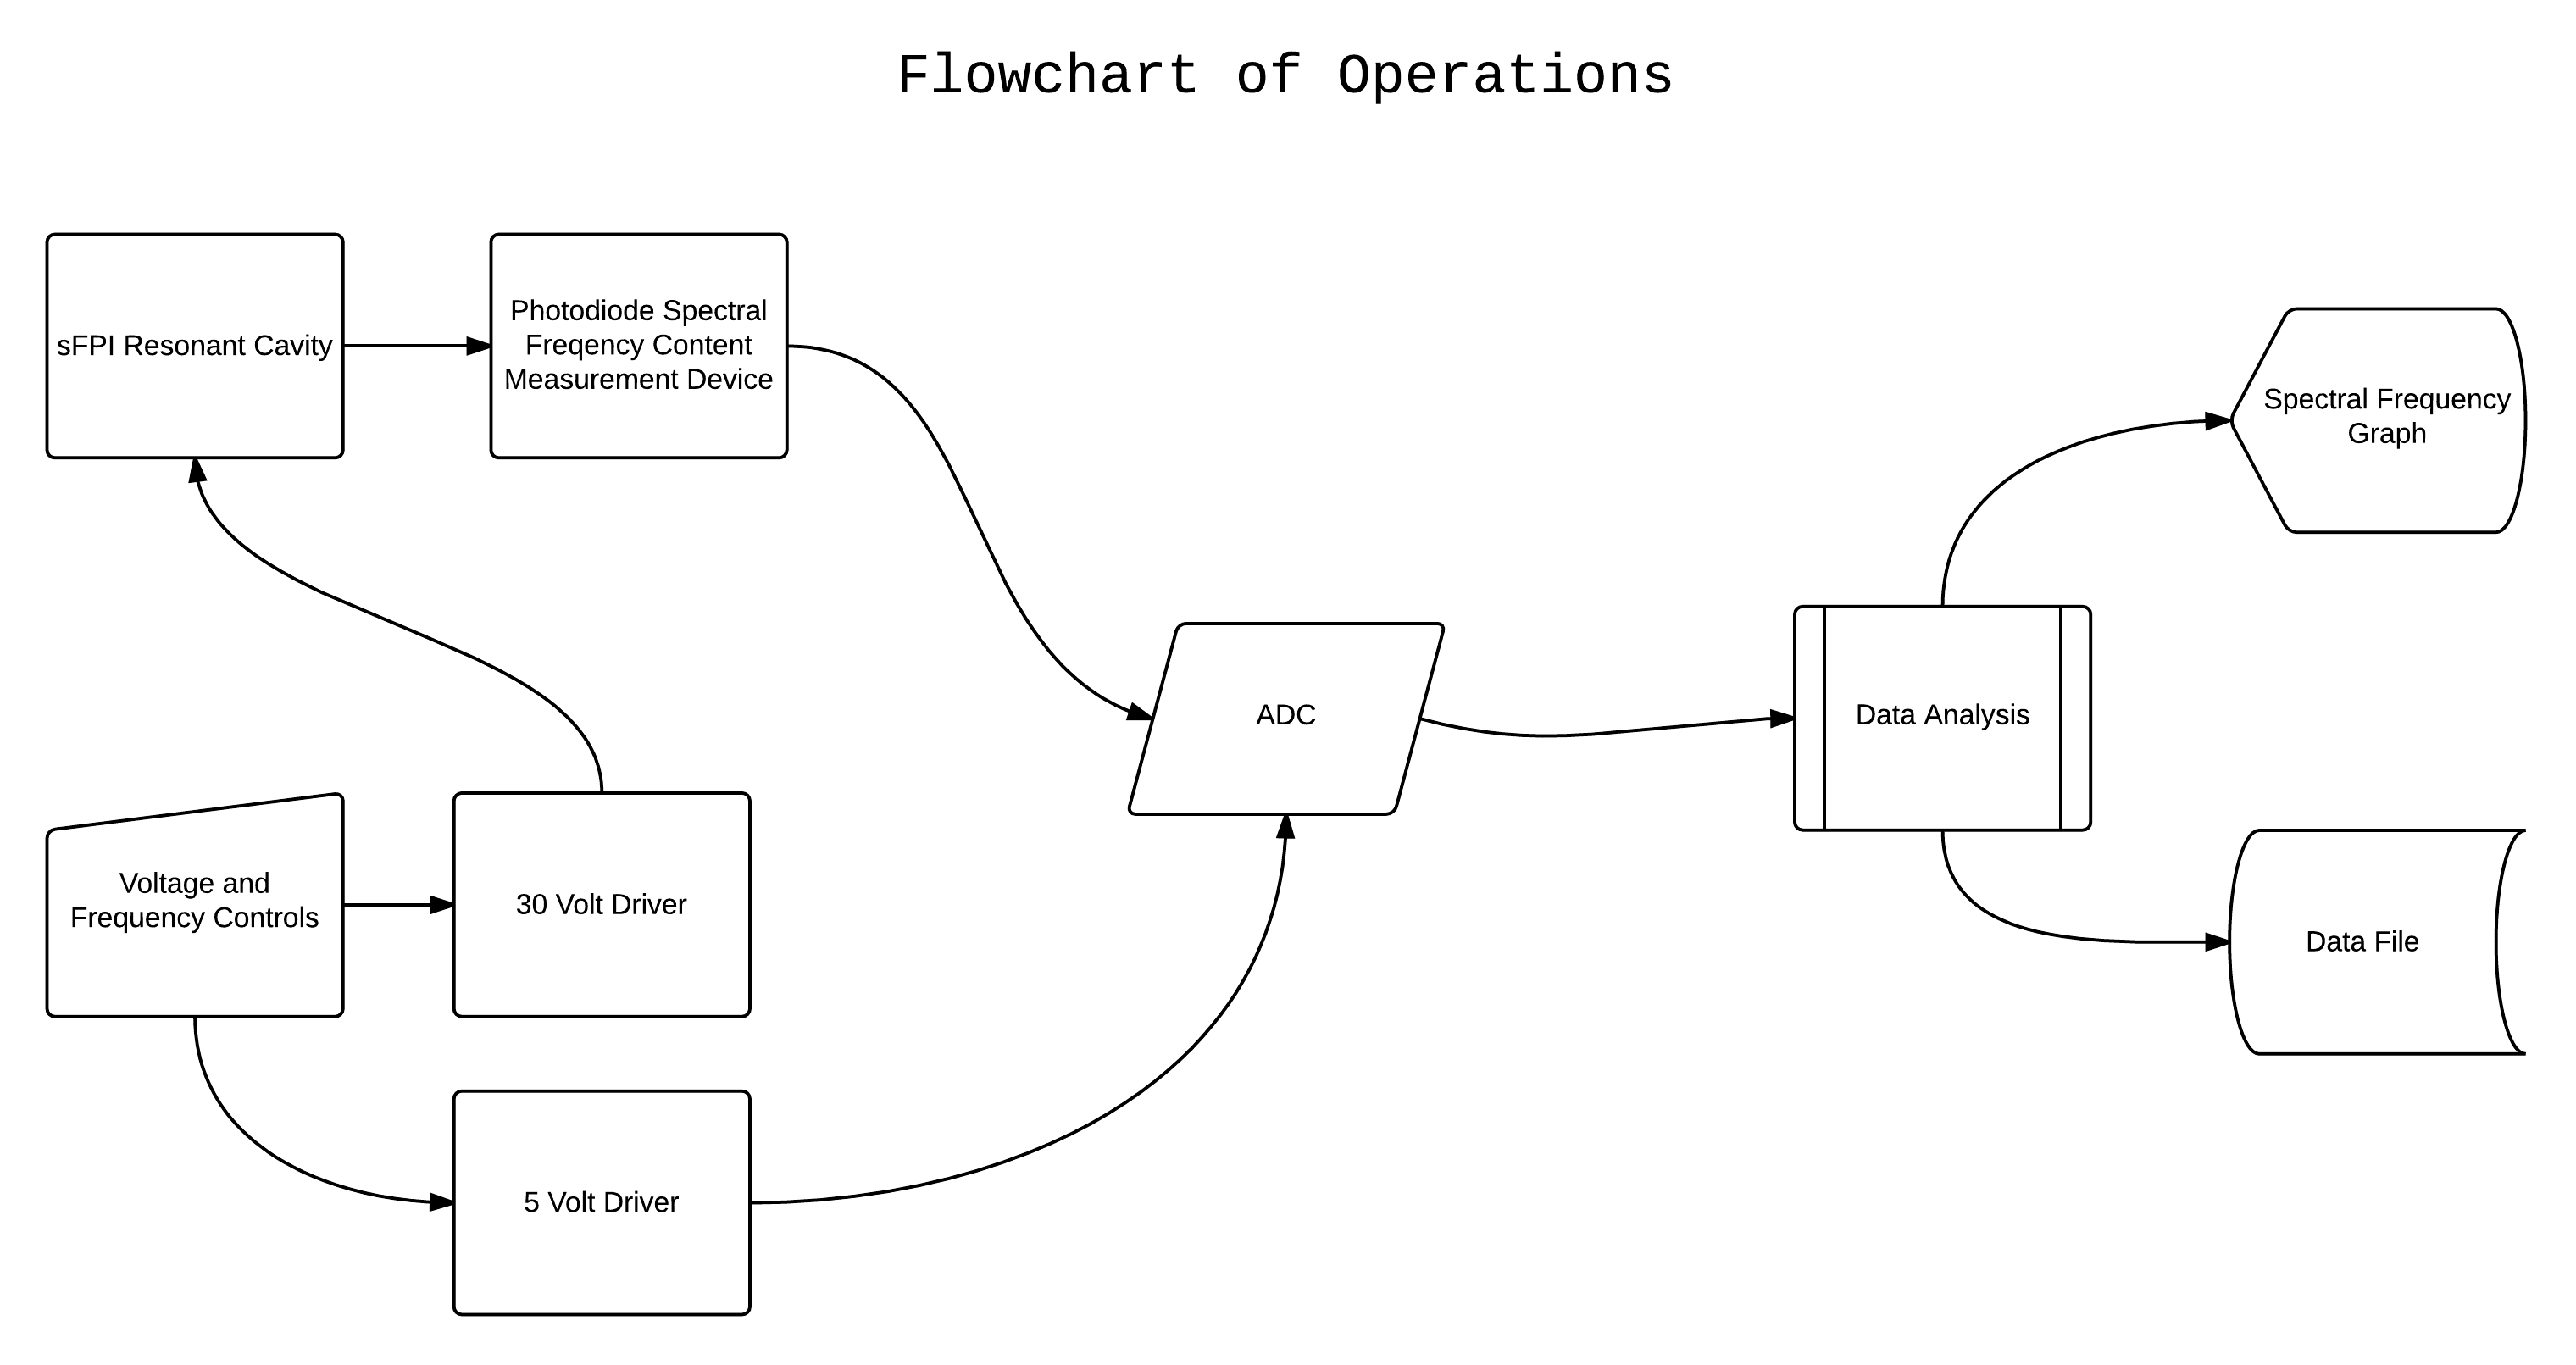
\includegraphics[width=6in]{block_diagram.png}
	\caption[Block Diagram]{Block Diagram of System Setup}
	\label{fig:block_diagram}
\end{figure}

% Optical Setup section

\section{Resonant Cavity}
The optical input as illustrated Figure~\ref{fig:block_diagram} above will consist of the sFPI. This delicate structure is an active system comprised of a two-confocal mirror resonant cavity, a piezoelectric device, and a photodiode.  The resonant cavity for the device is represented in Figure~\ref{fig:auxlens}. In order to determine the optimal distance between the lens and the first mirror, samples will be taken and the transmission peaks will be compared with those of the peaks of the SP-470-04 interferometer sample.

\begin{figure}[h!]
  \centering
	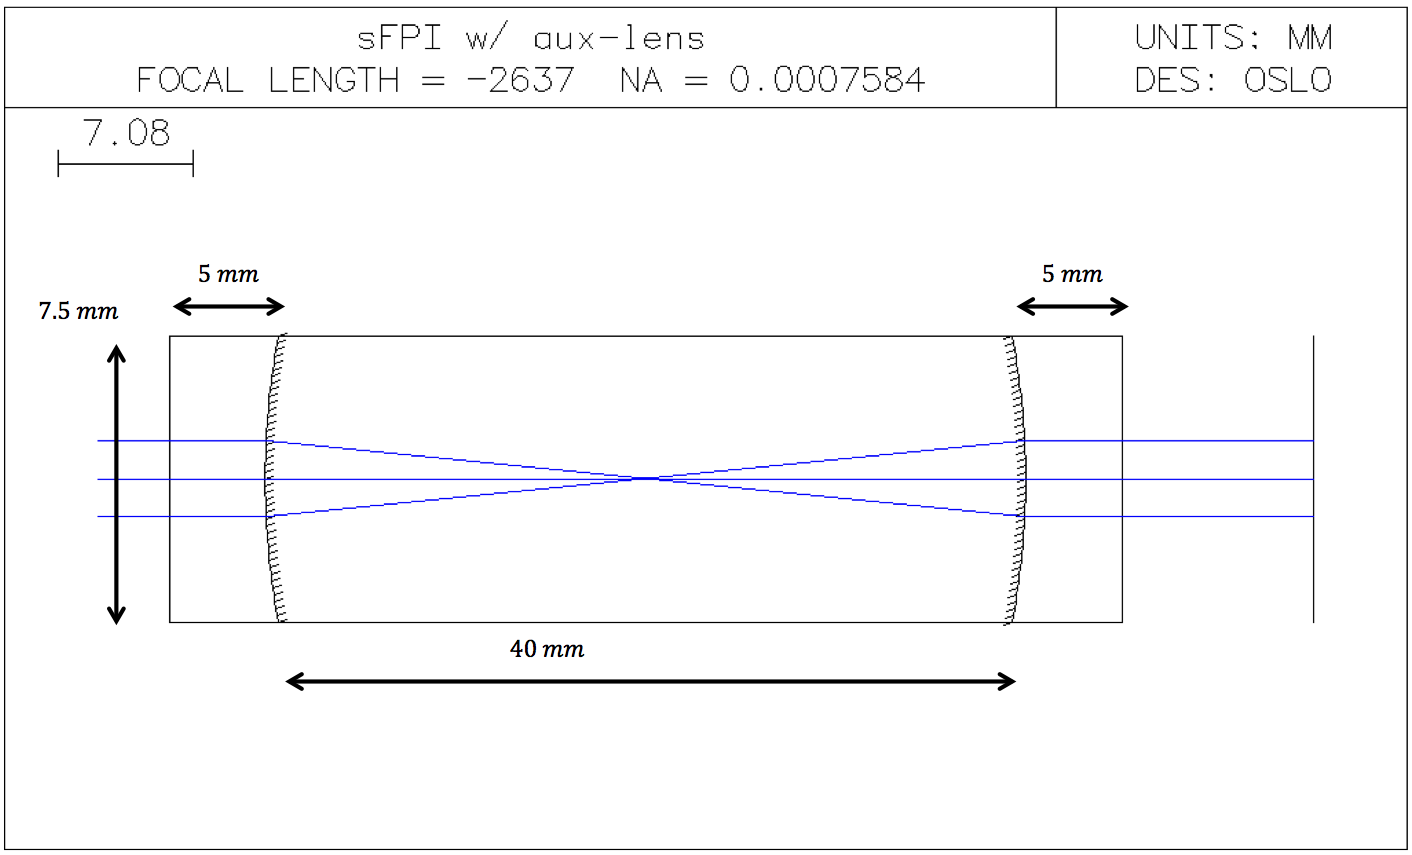
\includegraphics[width=5in]{sfpi_layout.png}\\
	\caption[Resonant Cavity Design]{The resonant cavity design, with measurements}
	\label{fig:auxlens}
\end{figure}

\begin{equation}
\Delta v = c/2L
\label{fsr}
\end{equation}

\begin{equation}
\Delta \delta = \Delta v/F^*
\label{bandwidth}
\end{equation}

The finesse of the sFPI is calculated based on the reflectivity of the mirrors (Eq.~\ref{finesse})~\cite{website}. The FSR of the resonant cavity of the sFPI is determined by Eq.~\ref{fsr} and the bandwidth is calculated by Eq.~\ref{bandwidth}~\cite{jenkinsnwhite}~\cite{optics}. The lens system will be held in place by a setup which holds the two spherical mirrors 40 mm apart and the auxiliary lens to promote maximum transmission of the modes (Figure~\ref{fig:lensholder}). Table~\ref{rescav} details the design specifications for the resonant cavity.

\begin{table}[!htpb]
\begin{center}
\begin{tabular}{*3c}
\toprule 
  Quantity & Minimum & Maximum \\ 
  \midrule 
  $L$ & \multicolumn{2}{c}{40 mm}\\  
  $\Delta v$ & \multicolumn{2}{c}{3.748 GHz}\\
  $R$ & $95 \%$ & $98\%$\\           
  $F^*$ & 61 & 155 \\
  $\Delta \delta$ & 61.2 MHz & 24.2 MHz\\
  \bottomrule 
\end{tabular}
\caption{Design Specification for Resonant Cavity}
\label{rescav}
\end{center}
\end{table}

The length of the resonant cavity will be adjustable for calibration purposes. After calibration, the length and origination of the cavity will remain constant. However, the angle of incidence as determined by the auxiliary focusing lens, will be variable so as to position for maximum transmission. 

\begin{figure}[h!]
	\centering
	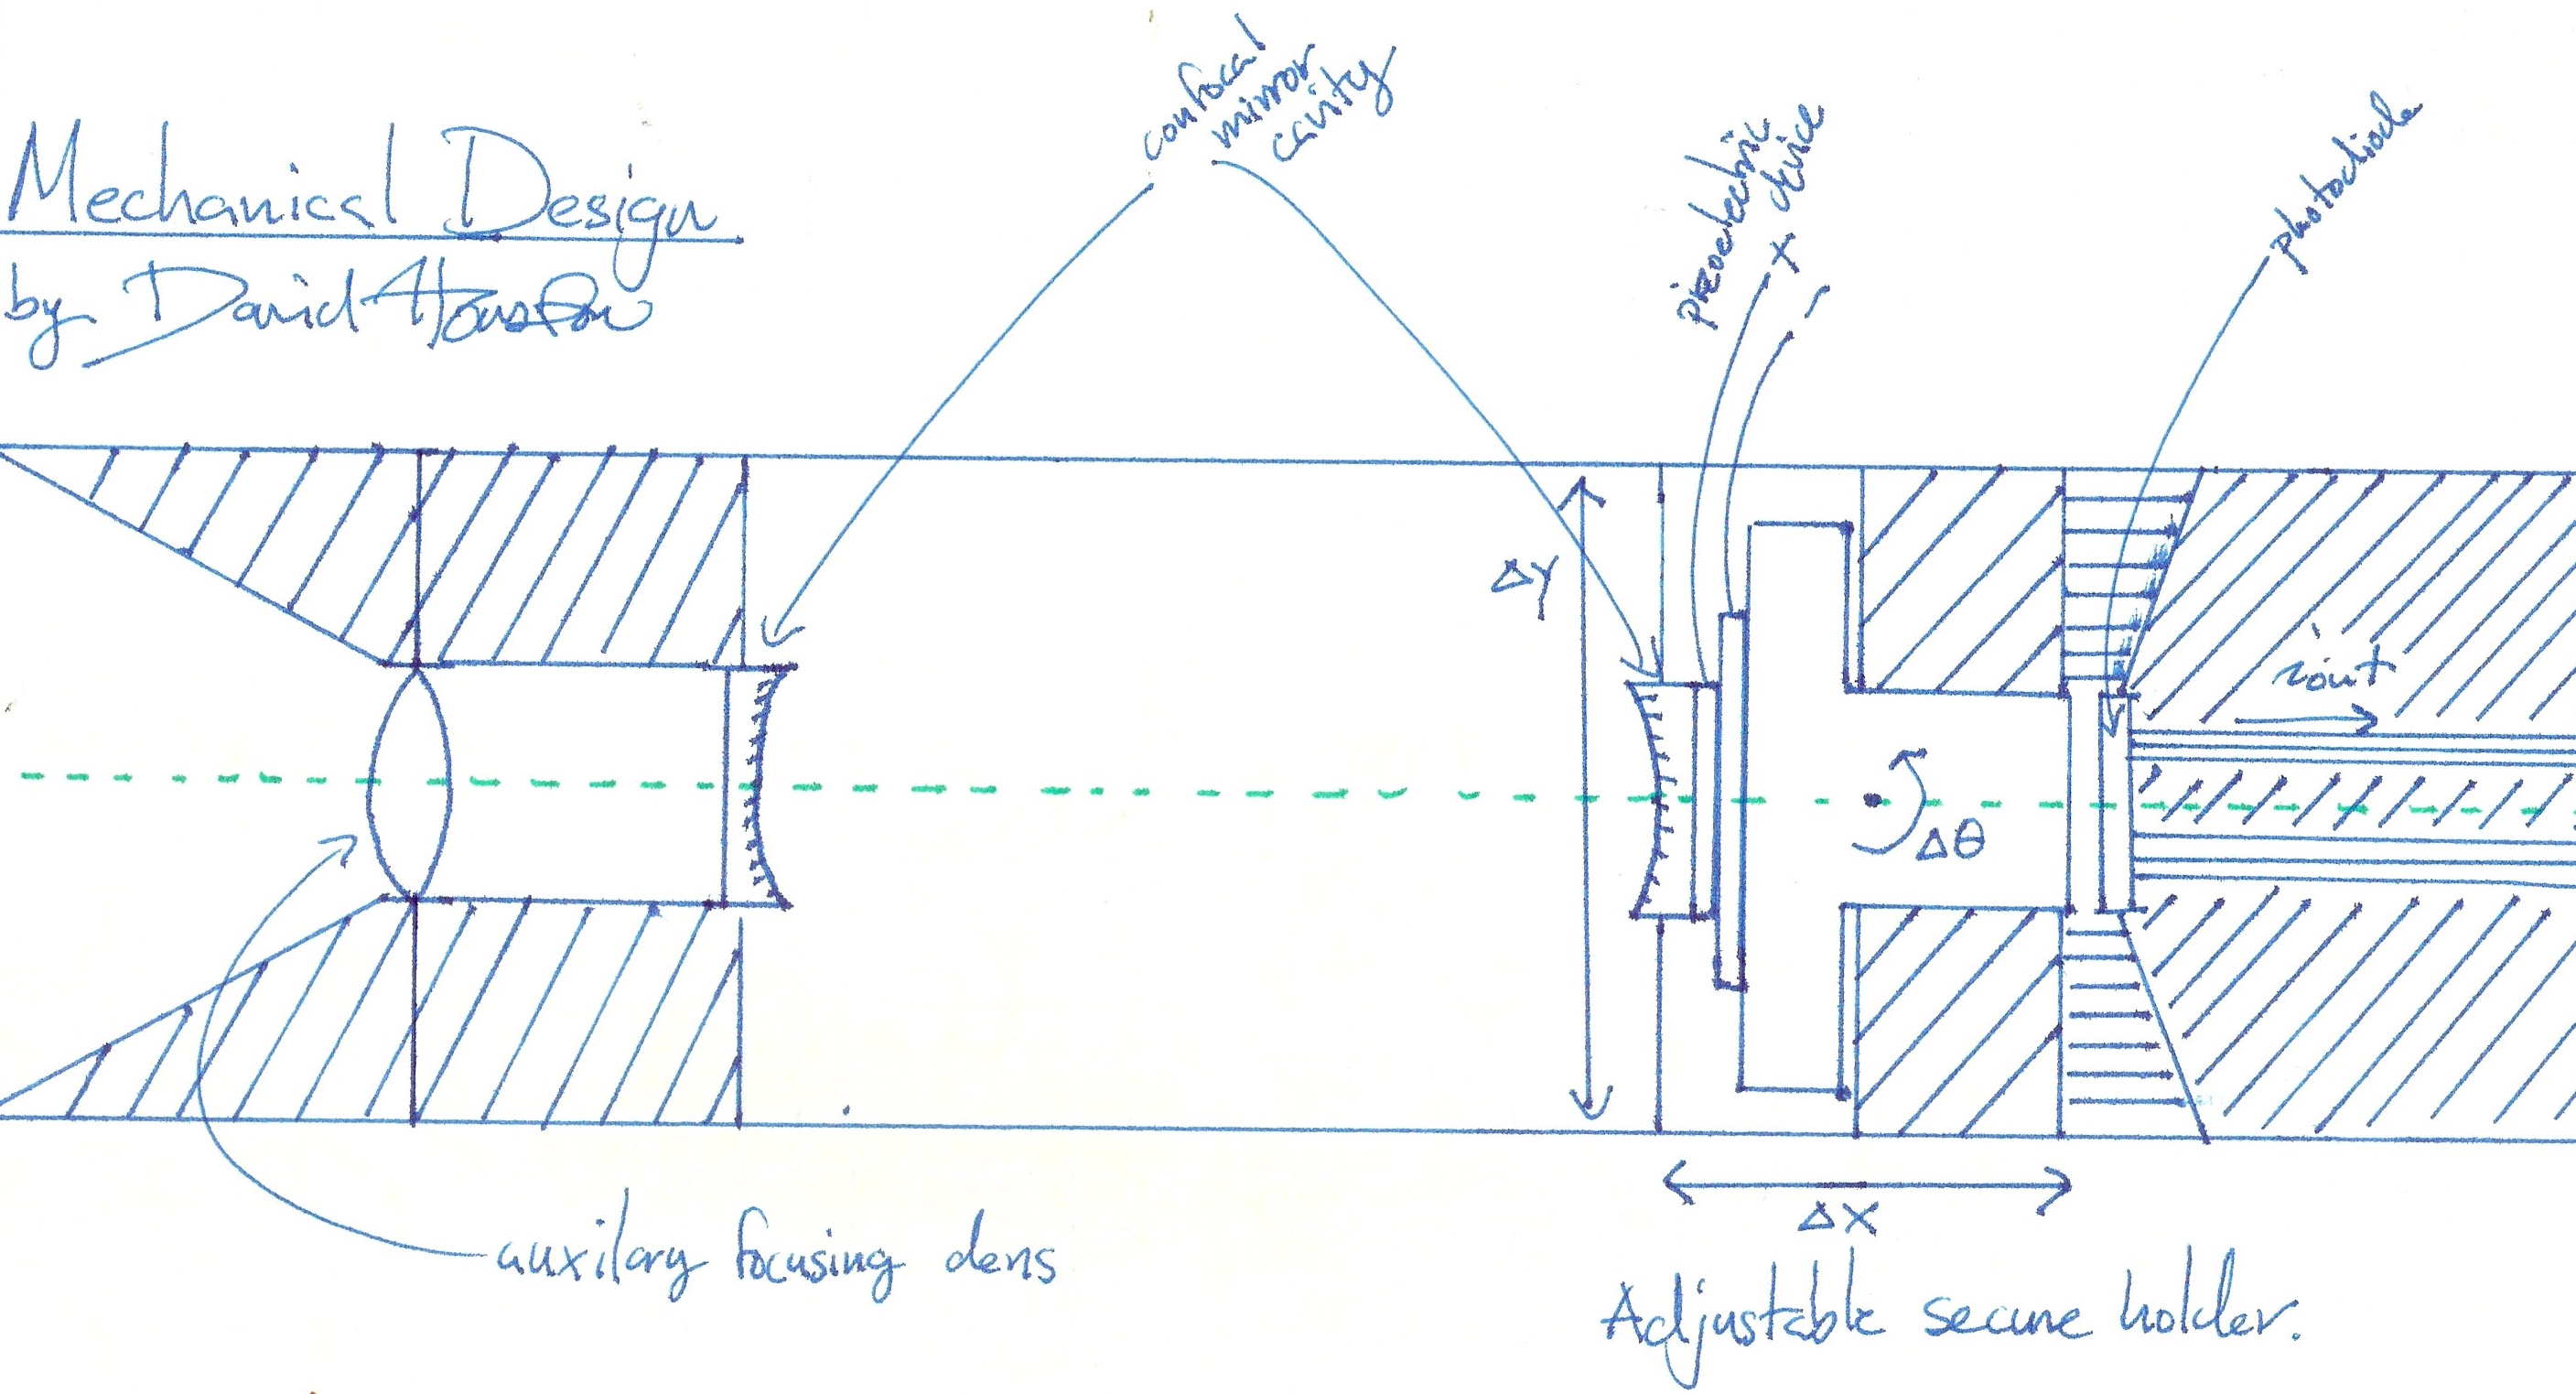
\includegraphics[width=\textwidth]{holder.jpeg}
	\caption{Resonant Cavity Mechanical Design}
	\label{fig:lensholder} 
\end{figure}

\section{The Driver}
The driver will be constructed using an Arduino UNO micro-controller. The Arduino UNO will take in a set of analog signal values in order to control the output. These analog signals will be attenuated DC voltage levels ranging from 0-5V. The bit resolution for the ADC is 10 bits, which twill allow for $2^{10}$ (or 1024) individual definable levels for the controls. The characteristics that will be controllable are the amplitude, time on, and the DC offset. These analog signals will be converted into digital signals, averaged every data cycle, and analyzed by the Arduino. The values will correspond to writeable outputs, which the Arduino will send to the DAC via I2C. The DAC will produce a 5V sawtooth voltage signal with a bit resolution of 1.2 mV/bit (Figure~\ref{fig:rampfunc}). 

% Stair Step Ramp Function Graph
\begin{figure}[h!]
 \centering
 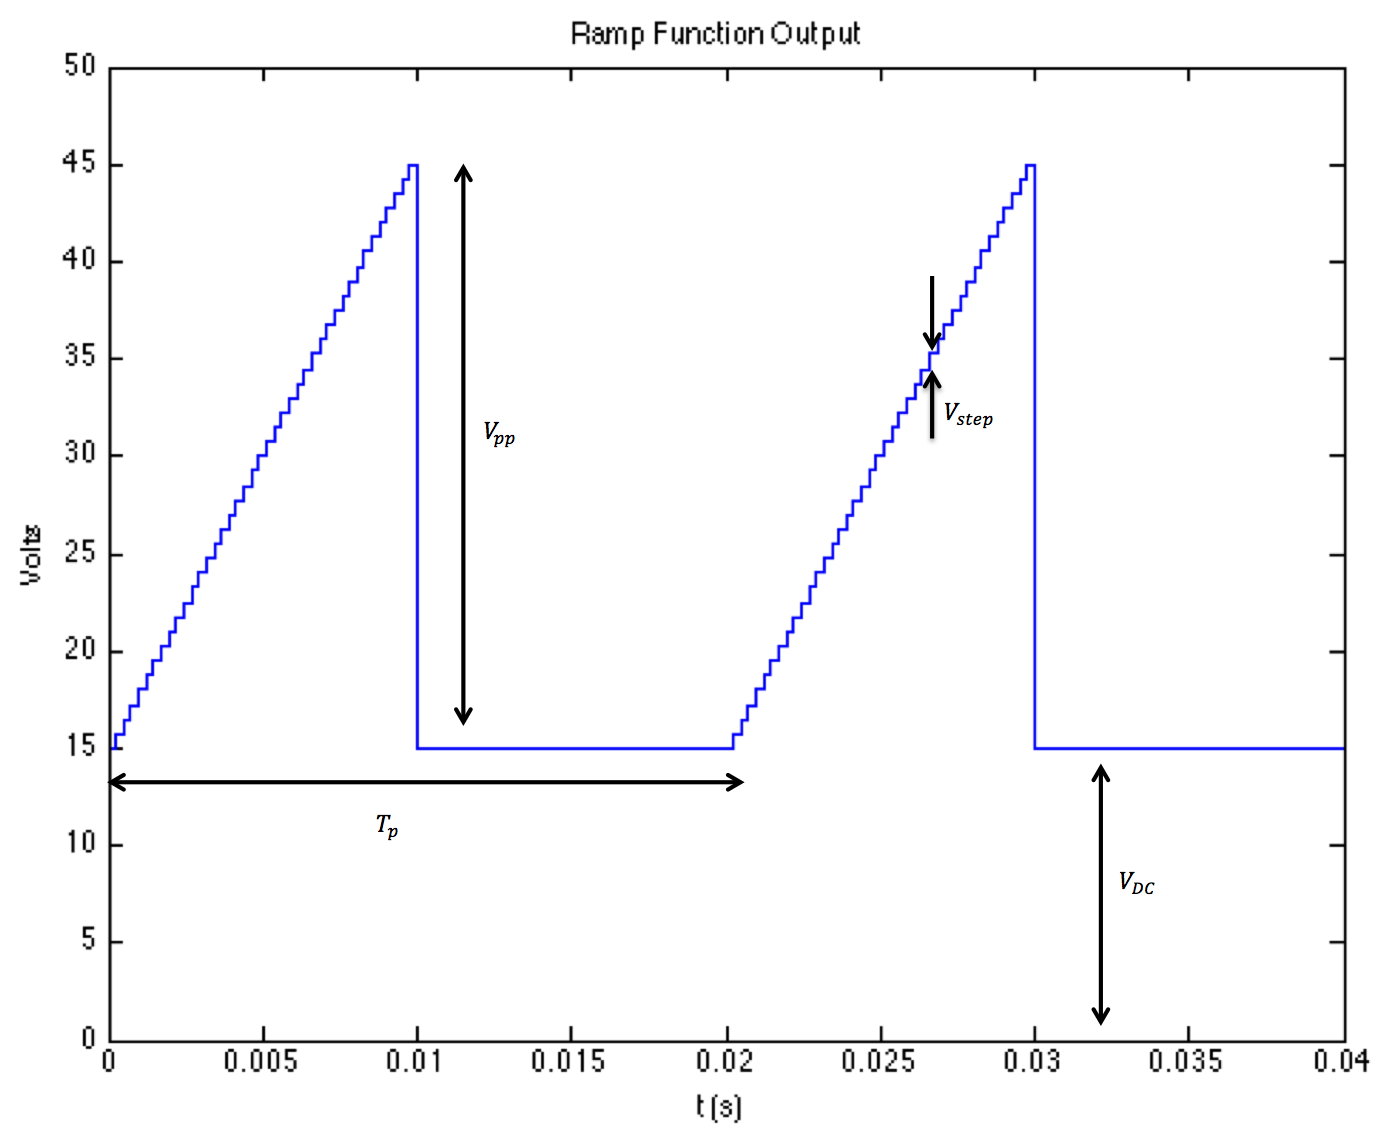
\includegraphics[width=4in]{stair_step_ramp_function.png}
 \caption[Ramp Function]{Graphical Representation of the Stair Step Ramp Function}
 \label{fig:rampfunc}
 \end{figure}

The frequency of the signal will be controlled by the value from the analog input and will only change the amount of time the signal is on (Eq.~\ref{freqramp}) The off, or rest, time is determined by the photodiode. The photodiode will be tested to determine the discharge time by measuring the time constants in a circuit configuration (Figure~\ref{fig:rctest}). 

\begin{equation}
f_r=(t_{on}+t_{off} )^{(-1)}
\label{freqramp}
\end{equation}

\begin{figure}[h!]
	\centering
	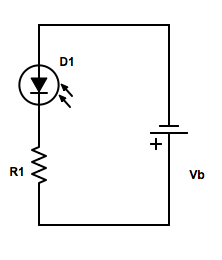
\includegraphics[width=2in]{diode_circuit.png}
	\caption[RC Diode Circuit]{Setup for measuring decay constant of the photodiode}
	\label{fig:rctest}
\end{figure}
  
The 5V sawtooth wave function will be fed to a filtered amplifier to amplify the signal based on a series-shunt feedback loop (Figures~\ref{fig:sawamp},~\ref{fig:rlcfilter}). Table~\ref{driverspecs} list the specifications for the amplifier\footnote{These values were taken by measuring the impedance of the piezoelectric device}.\newline

\begin{table}[!htpb]
\begin{center}
\begin{tabular}{*3c}
\toprule 
  Quantity & Value (50 Hz) & Value (100 Hz)\\ 
  \midrule                   
  $A_{cl_{max}}$ & \multicolumn{2}{c}{$7 V/V$} \\
  $A_{cl_{min}}$ & \multicolumn{2}{c}{$0.1 V/V$} \\
  $f_{c}$ & \multicolumn{2}{c}{200 Hz} \\
  $Z_{load}$ & $370 - j2.0499*10^5 \;\Omega$ & $370- j1.0250*10^5 \;\Omega$\\
  $Z_{out}$ & $370 + j2.0499*10^5 \;\Omega$ & $370 + j1.0250*10^5 \;\Omega$\\
  \bottomrule 
\end{tabular}
\caption{Design Specifications for Driver Amplifier of 5V sawtooth wave at 50 and 100 Hz}
\label{driverspecs}
\end{center}
\end{table}
 
 % Driver Amplifier
 \begin{figure}[h!]
 \centering
 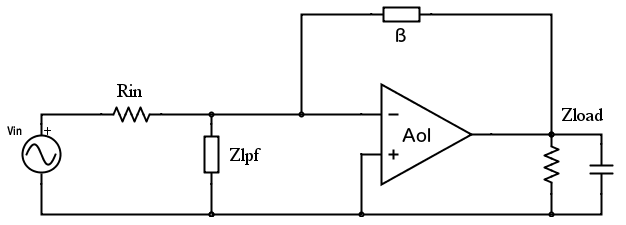
\includegraphics[width=6in]{driver_amp.png}
 \caption[Driver Amplifier]{$1^{st}$ Order Driver Amplifier for 5V Sawtooth Wave}
 \label{fig:sawamp}
 \end{figure}

% RC Filter
\begin{figure}[h!]
\centering
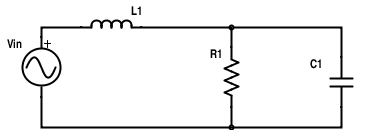
\includegraphics[width=4in]{rlc_filter.png}
\caption[RLC Filter]{RLC Filter}
\label{fig:rlcfilter}
\end{figure}

\noindent The Arduino--DAC-Amplifier component will have an impedance as described in Eq.~\ref{pmax} and rated to 60 mW when the Thevinin impedance of the circuit is equivalent to the load impedance of piezoelectric device.
 
\begin{equation}
P_{max} \sim Z_{th} = Z^*_{load}
\label{pmax}
\end{equation}

Table~\ref{finalsignal} details the specifications of the the final signal delivered to the piezoelectric device. 
% Specifications for the Driver
\begin{table}[h!]
\begin{center}
\begin{tabular}{*3c}
\toprule 
  Quantity & Minimum & Maximum \\ 
  \midrule                   
  $V_{pp}$ & 0.5 V & $30$ V  \\
  $V_{dc}$ & 0 V & $30$ V  \\
  $V_{step}$ & $122\; \mu V$ & $1.2$ mV \\
  $f$ & 50 Hz & $100$ Hz  \\
  \bottomrule
\end{tabular}
\caption{Specifications for sFPI Driver Output Signal}
\label{finalsignal}
\end{center}
\end{table}
 
\section{The Processor}
The photodiode will be mounted to an adjustable plate at the rear of the sFPI for calibration, for maximum transmission of the spectral content. The photodiodes resulting current will be reverse biased and amplified by a transimpedance negative-feedback amplifier (Figure~\ref{fig:photodiode}). Table~\ref{processorspecs} details the specifications for the shunt-shunt transimpedance photodiode amplifier.

\begin{figure}[h!]
\centering
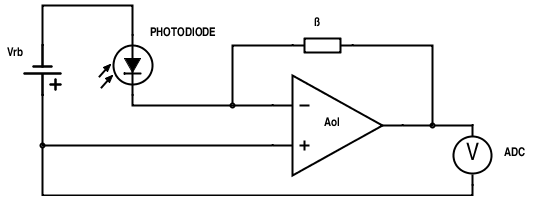
\includegraphics[width=4in]{photodiode_transimp_amp.png}
\caption[Photodiode Output Circuit]{Reverse Biased Transimpedance Amplifier of the Photodiode output}
\label{fig:photodiode}
\end{figure}

\begin{table}[!htpb]
\begin{center}
\begin{tabular}{*3c}
\toprule 
  Quantity & Minimum & Maximum \\ 
  \midrule                   
  $V_{ADC}$ & 0 V & 5 V \\
  $A_{CL}$ & \multicolumn{2}{c}{$A_{OL}/(1+A_{OL}\beta)$ V/A}\\
  \bottomrule
\end{tabular}
\caption{Design Specifications for Photodiode Transimpedance Amplifier.}
\label{processorspecs}
\end{center}
\end{table}

\section{The Digital Output}
The content captured by the ADC (Figure~\ref{fig:photodiode}) will be transmitted to a computer to process, display (by a graphical representation), and store the data. This data will be combined in conjunction with the 5V sawtooth signal to plot the photodiode signal as a function of the geometrical change of the resonant cavity, which is proportional to the wavelength of the light. This will be done via a GUI model with a language that possesses the capability for universal interfacing. Python will be the base model for programming; however, other languages will be tested for user interface and compared based on speed, cross-platform configuration, and simplicity.

%\section{Evaluation}
\chapter[Evaluation]{The Evaluation of the sFPI}
The resonant cavity will have a Finesse of $155 \pm 1$ a FSR of $3.75 \pm 0.1$ GHz and a bandwidth of $24 \pm 0.1$ MHz. This will be tested by (See Finesse Measure PDF). To test the sFPI driver, the system will be setup with an output to a piezoelectric load and the voltage will be measured at different settings of the device. It will have a maximum peak-to-peak voltage of $30 \pm 0.01 V$, a maximum DC voltage of $30 \pm 0.01 V$, a maximum bit voltage of $8.4 \pm 0.01$ mV, and  a frequency range of $50 - 100 \pm 0.1$ Hz. The final test will be to measure the spectral frequency content of a HeNe laser and comparing the corresponding graphical output to the output of a SP-470-04 Interferometer. The final results must be within $1\%$ of each other. 

%\section{Timeline}
\chapter[Timeline]{Explicit Timeline of the Proposed Project}
\begin{figure}[h!]
	\centering
	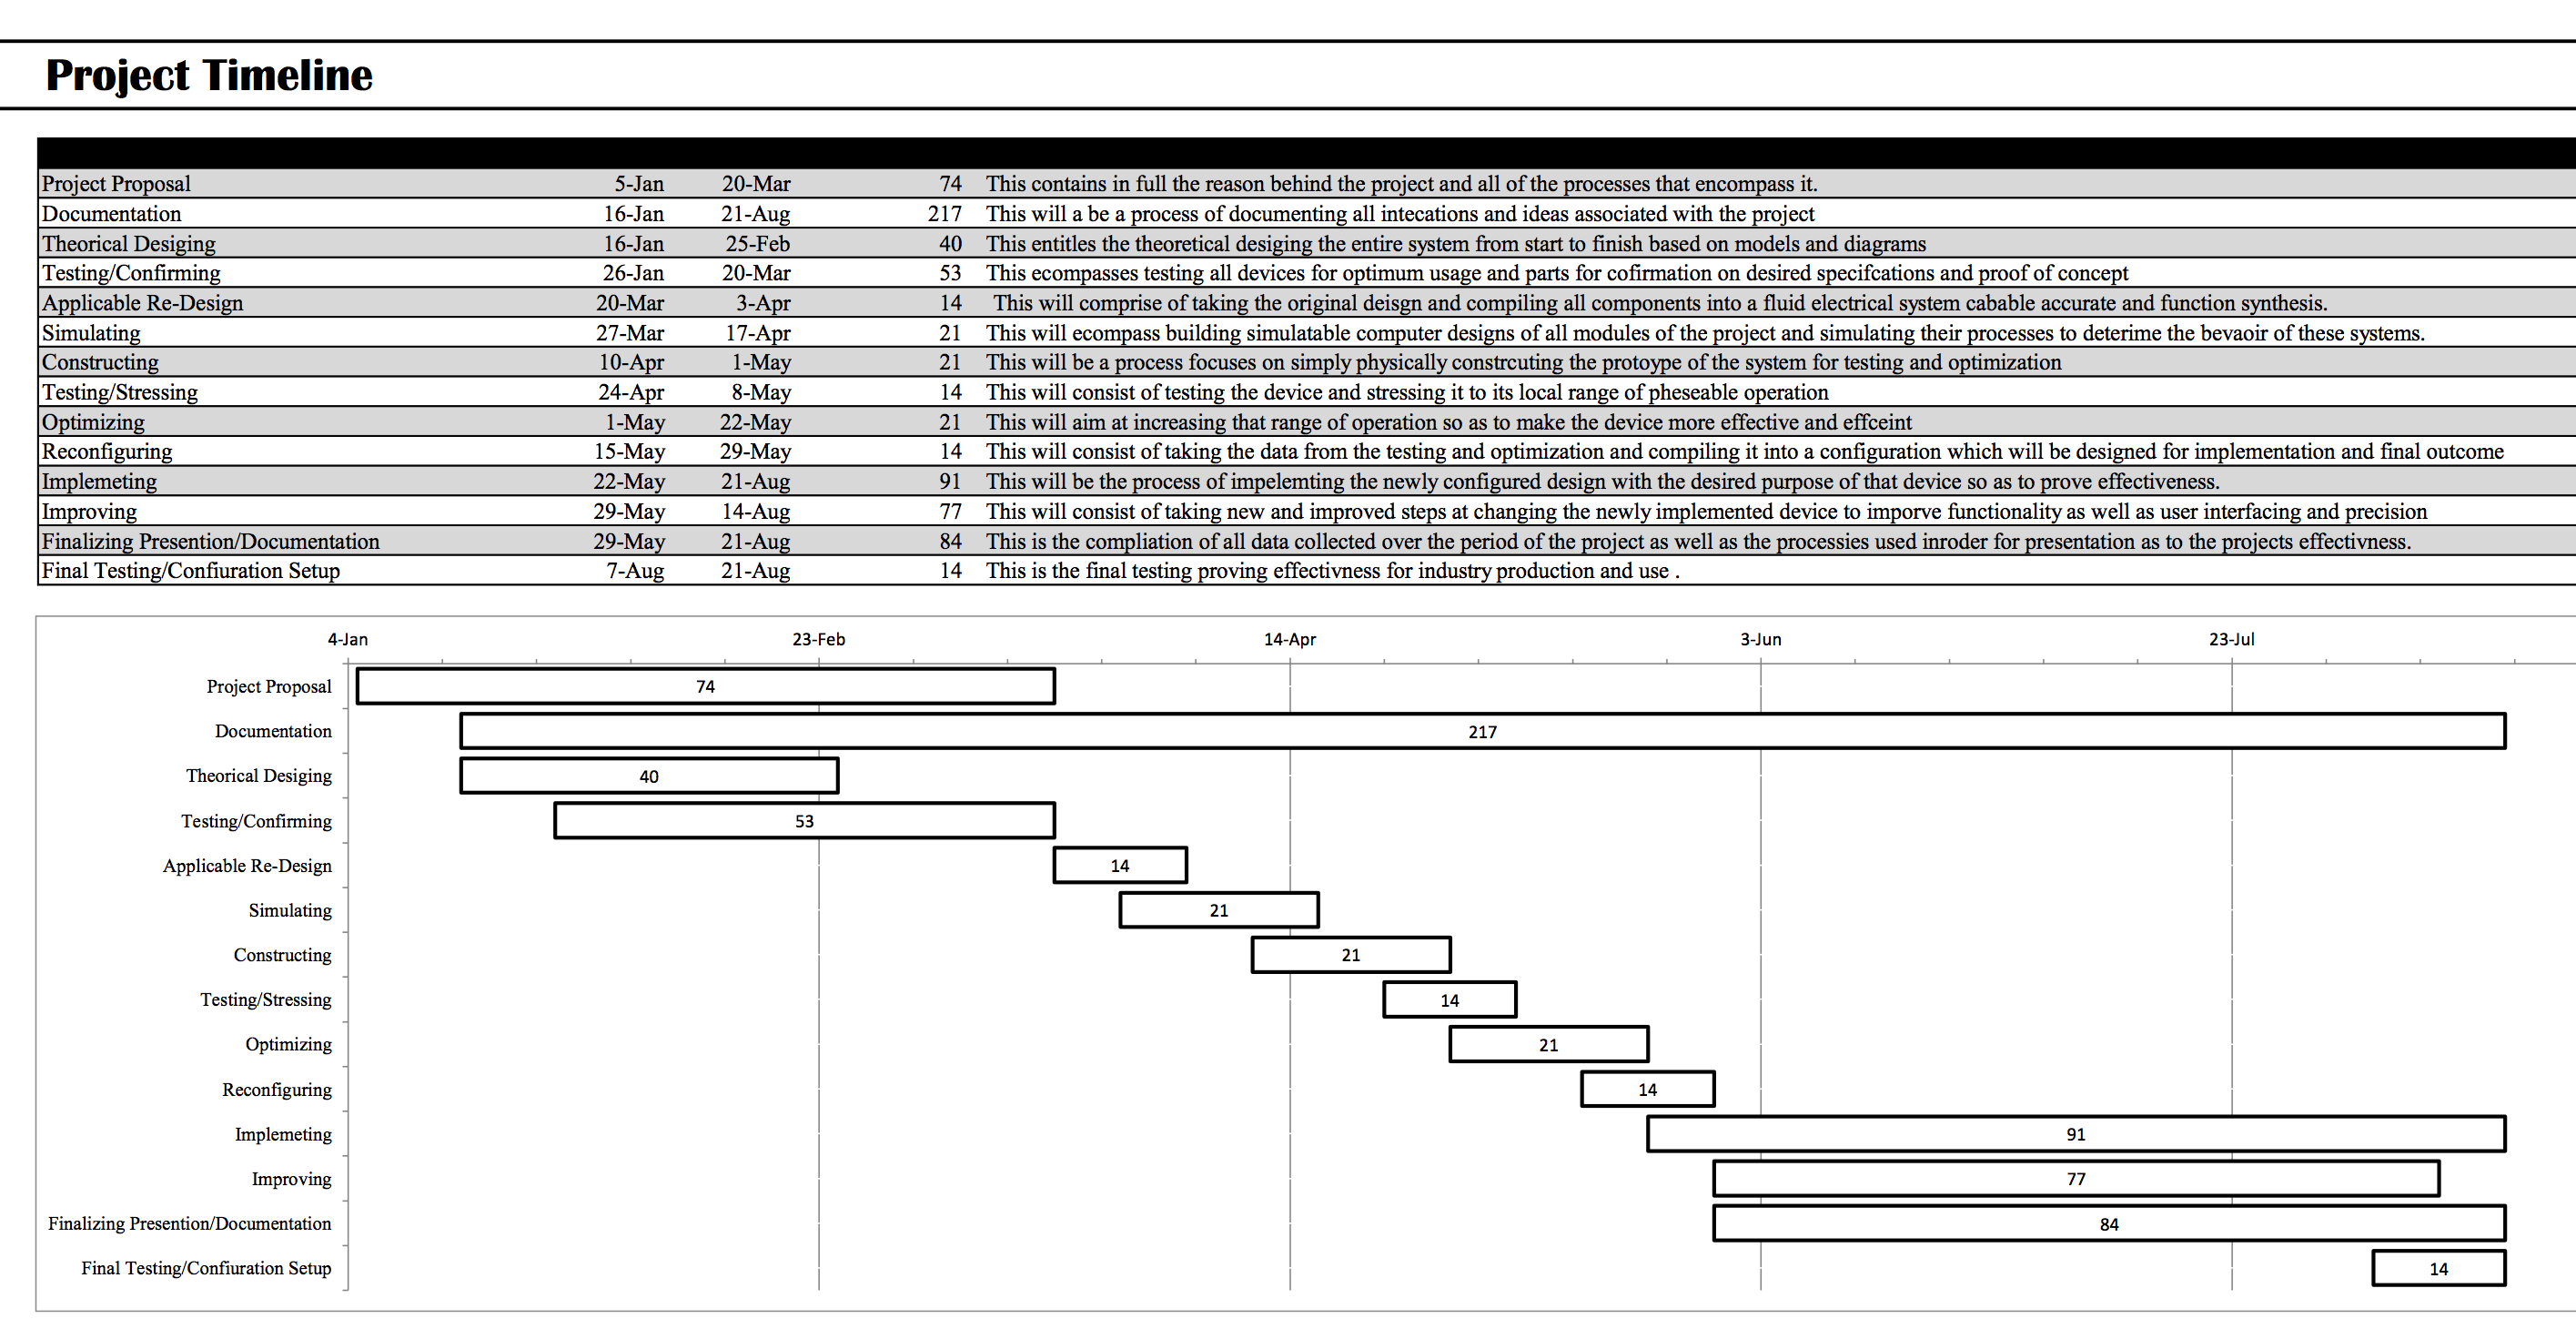
\includegraphics[width=\textwidth]{timeline.png}
	\caption{Timeline}
	\label{fig:timeline}
\end{figure}
 
\begin{appendices}
\chapter[Schematics]{}

\begin{sidewaysfigure}[h!]
  \centering
	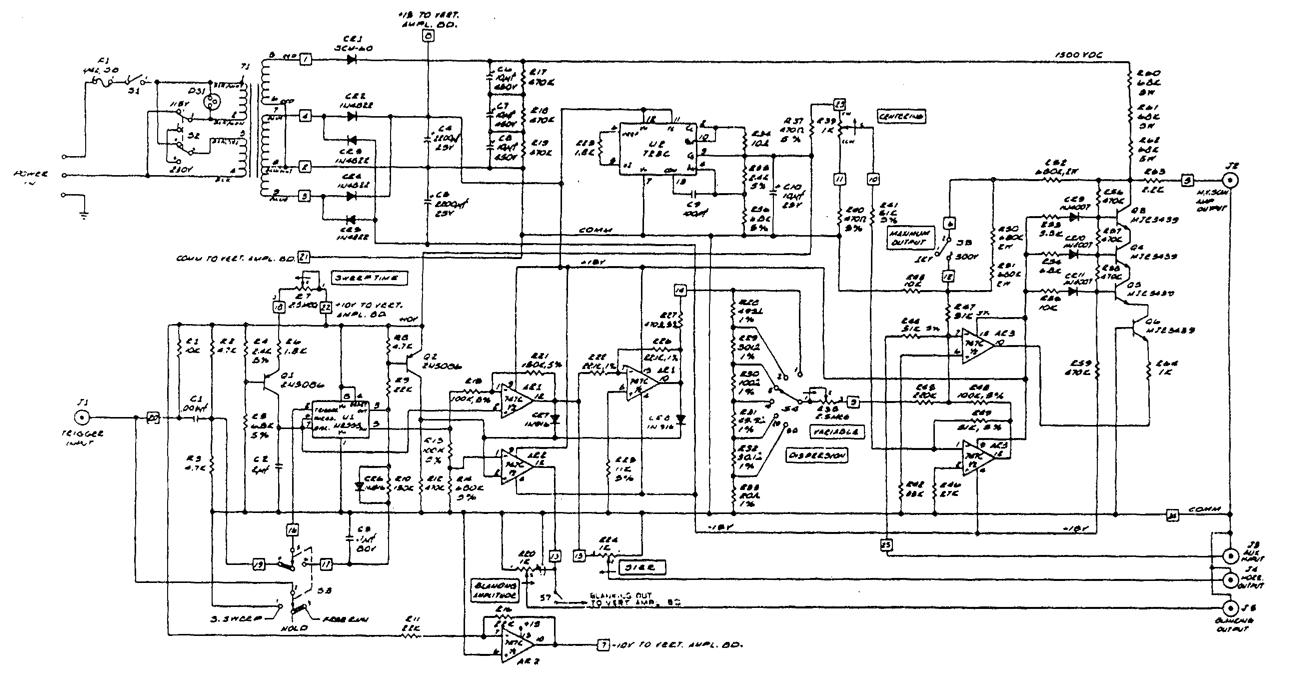
\includegraphics[width=\textwidth]{driver_schm.png}\\
	\caption[SP-476 Schematic]{SP-476 Schematic~\cite{sfpidriver}}
	\label{fig:driverschm}
\end{sidewaysfigure}

\begin{sidewaysfigure}[h!]
  \centering
	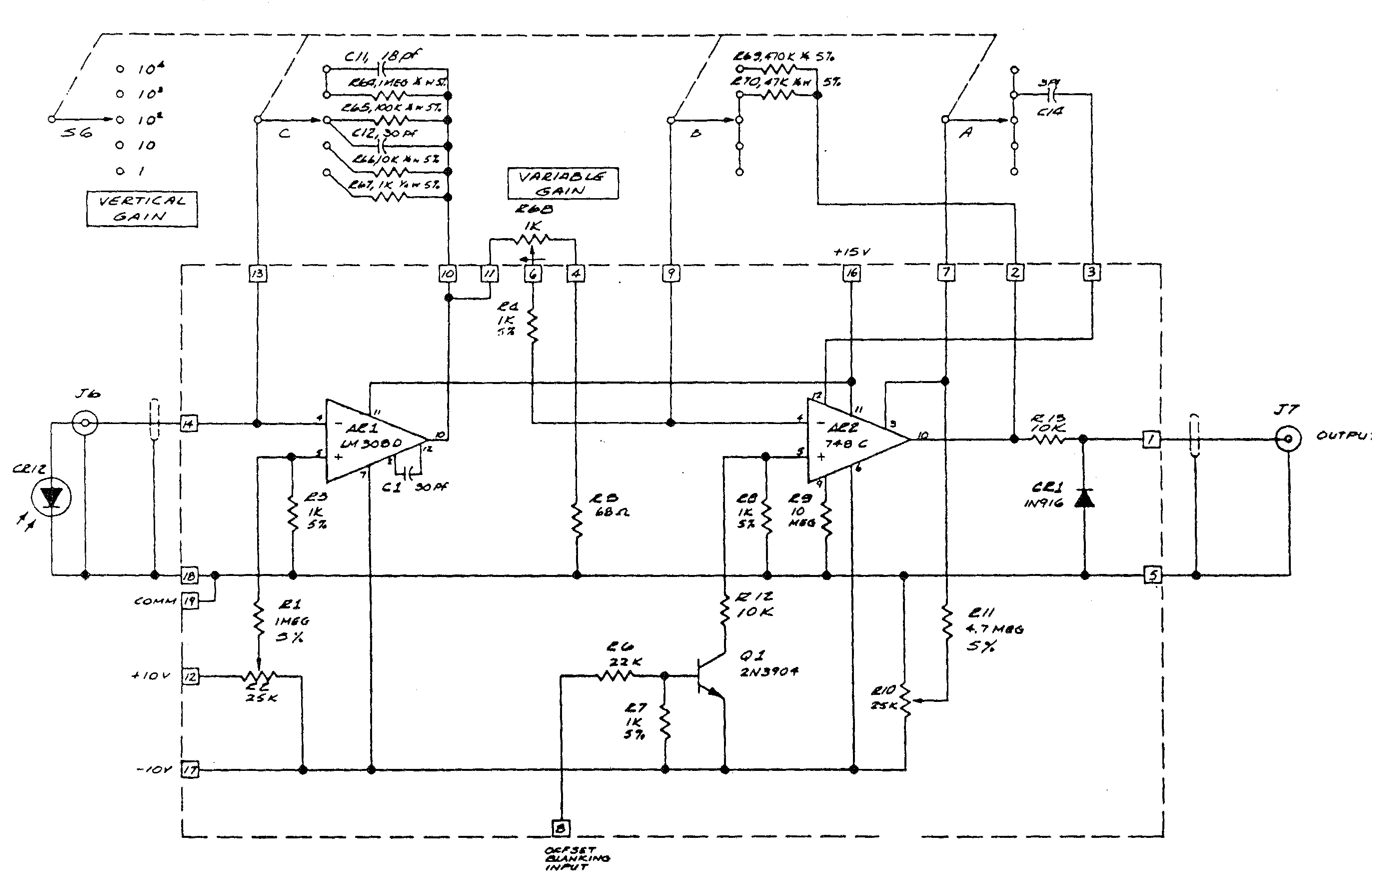
\includegraphics[width=\textwidth]{amp_schm.png}\\
	\caption[Amplifier Schematic]{Amplifier Schematic~\cite{sfpidriver}}
	\label{fig:ampschm}
\end{sidewaysfigure}

\end{appendices}

\bibliography{OIT_Thesis}
\printnomenclature
\end{document}